\documentclass[a4,paper,fleqn]{article}

\usepackage{layout}

\newcommand{\uuline}[1]{{\underline{\underline{#1}}}}

\title{AES - Übung 6 \\Auslegung einer netzgekoppelten PV-Anlage}
\date{\today}
\author{Daniel Winz}

\begin{document}
\maketitle
%\clearpage
\vfill
\tableofcontents
\vfill
\clearpage

\section{Ausgangslage}
Es ist eine Photovoltaikanlage für ein Flachdach ausgelegt werden. Dabei ist 
sowohl der Energieertrag als auch die Kosten berücksichtigt werden. 

\begin{figure}[h!]
    \centering
    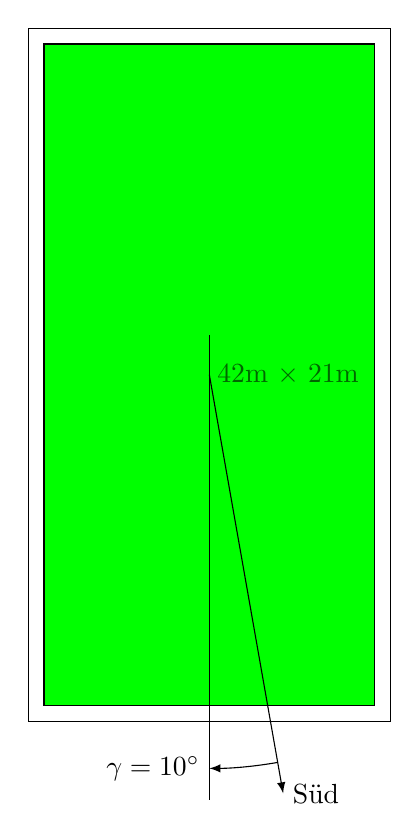
\begin{tikzpicture}[scale=0.2]
        \draw[] (-11.5,-22.0) rectangle (11.5,22.0);
        \draw[fill=green] (-10.5,-21.0) rectangle (10.5,21.0);
        \draw (0,2.5) -- (0,-27.0);
        \draw[-latex] (0,0) -- (280:27.0) node[right] {Süd};
        \draw[latex-] (0,-25.0) node[left] {$\gamma = 10^\circ$} 
            arc [start angle=270, end angle=280, radius=25.0];
        \node[green!40!black] at (5.0,0) {42m $\times$ 21m};
    \end{tikzpicture}
    \label{fig:roof}
    \caption{Geometrie und Ausrichtung des Flachdachs}
\end{figure}

\clearpage

\section{Layout}
Eine Drehung der Module nach Süden lohnt sich aufgrund des kleinen Winkels von 
$10^\circ$ nicht. 
\begin{figure}[h!]
    \centering
    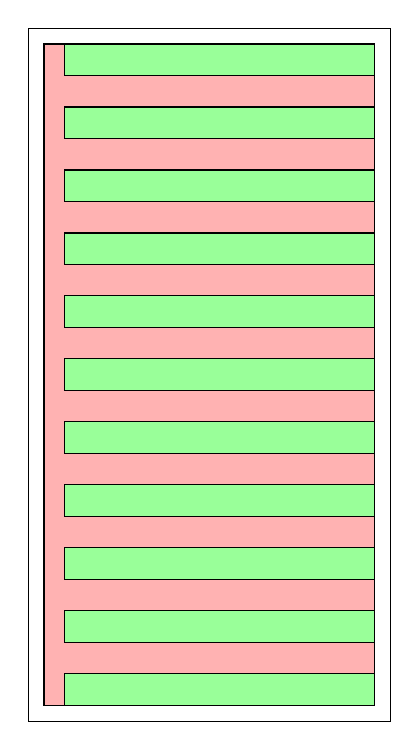
\begin{tikzpicture}[scale=0.2]
        \draw[] (-11.5,-22.0) rectangle (11.5,22.0);
        \draw[fill=red!30] (-10.5,-21.0) rectangle (10.5,21.0);
        \foreach \i in {-21,-17,...,21} {
            \draw[fill=green!40] (-9.2,\i) rectangle (10.5,\i+2);
        }
    \end{tikzpicture}
    \label{fig:layout_sketch}
    \caption{Layoutskizze}
\end{figure}

\section{Modulwahl}
Aufgrund des guten Preis/Leistungs Verhältnis wird das Panel C verwendet. Es 
ist das günstigste Panel in der gegebenen Auswahl und bietet einen 
vergleichsweise guten Wirkungsgrad. Panel D weist einen leicht höheren 
Wirkungsgrad auf, ist aber verglichen mit den anderen Modulen 
unverhältnismässig teuer. 

\section{Aufständerung}
Zur Ermittlung der Aufständerung wird eine Matlab Funktion geschrieben. Dieses 
ist in Anhang \ref{app_panelize} ersichtlich. Die Funktion muss mit den 
Parametern Dachabmessungen, Panelgrösse, Aufstellwinkel, Freiwinkel und 
minimaler Abstand zwischen den Panels aufgerufen werden. Die Funktion 
ermittelt dann die optimale Aufstellung der Panels auf dem Dach. 

\noindent
Diese Funktion wird nun mit einem Matlab Skript (Anhang \ref{app_panels}) mit 
verschiedenen Aufstellwinkeln aufgerufen. Zudem wird die vertikale und die 
horizontale Montage der Panels berücksichtigt. Aus diesen Daten werden 
anschliessend Leistungsabgabe und Panelkosten berechnet. Diese können mit 
Gewichtungsfaktoren (Zeilen 95 und 96) unterschiedlich gewichtet werden. Mit 
diesen wird nun die optimale Aufstellung der Panels ermittelt. Anschliessend 
wird der Ertrag und die Kosten der Anlage berechnet. Dazu müssen die Inverter 
und Anschlusskästen von Hand parametrisiert werden. (Zeilen 185, 189, 193 und 
197 $\to$ Wechselrichter und Zeilen 210, 212 und 214 $\to$ Anschlusskästen)

\section{Ausgaben}
\subsection{Plots}
\begin{figure}[h!]
    \centering
    \includegraphics[width=0.6\textwidth]{nof_panels.pdf}
    \label{fig:nof_panels}
    \caption{Anzahl Panels abhängig vom Aufstellwinkel}
\end{figure}
\begin{figure}[h!]
    \centering
    \includegraphics[width=0.6\textwidth]{leftover.pdf}
    \label{fig:leftover}
    \caption{Unnötig ungenutzte Länge abhängig vom Aufstellwinkel}
\end{figure}
\begin{figure}[h!]
    \centering
    \includegraphics[width=0.6\textwidth]{total_radiation.pdf}
    \label{fig:total_radiation}
    \caption{Bestrahlung abhängig vom Aufstellwinkel}
\end{figure}
\begin{figure}[h!]
    \centering
    \includegraphics[width=0.6\textwidth]{power_cost.pdf}
    \label{fig:power_cost}
    \caption{Leistung pro Franken abhängig vom Aufstellwinkel}
\end{figure}
\begin{figure}[h!]
    \centering
    \includegraphics[width=0.6\textwidth]{weight_result.pdf}
    \label{fig:weight_result}
    \caption{Ergebnis nach Gewichtung mit Gewichtungsfaktoren 1 für Leistung 
        und 7 für Kosten abhängig vom Aufstellwinkel}
\end{figure}

\clearpage
\subsection{Terminalausgabe}
\lstinputlisting{example_output.txt}

\section{Anschluss}
Es werden jeweils 20 Panels in Serie zusammengefasst. Diese Stränge werden 
direkt an Wechselrichter vom Typ C angeschlossen. Die Wechselrichter werden 
mit einem Anschlusskasten vom Typ 3 ans Netz angeschlossen. 

\section{Ergebnisse}
\begin{zebratabular}{
    p{0.10\textwidth}
        p{0.10\textwidth}
        p{0.07\textwidth}
        p{0.07\textwidth}
        p{0.08\textwidth}
        p{0.11\textwidth}
        p{0.11\textwidth}}
    \rowcolor{gray}
    Gewichtung Leistung &
        Gewichtung Kosten &
        Anzahl Panels &
        Anzahl WR\_C &
        Jährliche Energie kWh &
        Kosten [CHF/kWh] &
        Ertrag [kWh/CHF] \\
    1 &
        9 &
        240 &
        4 &
        57.2 &
        0.213 &
        4.69 \\
    1 &
        8 &
        260 &
        5 &
        58.7 &
        0.233 &
        4.30 \\
    1 &
        5 &
        280 &
        5 &
        60.5 &
        0.236 &
        4.23\\
    1 &
        3.5 &
        300 &
        5 &
        62.3 &
        0.240 &
        4.17 \\
    1 &
        3.2 &
        320 &
        6 &
        64.2 &
        0.256 &
        3.91 \\
    1 &
        3 &
        340 &
        6 &
        66.2 &
        0.258 &
        3.88 \\
    1 &
        2.5 &
        380 &
        7 &
        69.1 &
        0.278 &
        3.60 \\
\end{zebratabular}

\section{Ablage}
Die im Rahmen dieser Arbeit erstellten Skripte sind auf Github verfügbar: \\
\url{https://github.com/daniw/aes/tree/master/sw06}

\clearpage
\begin{appendix}
\section{Daten Solarpanels}
\begin{zebratabular}{lllll}
\rowcolor{gray}
Solarmodul &
    PV\_A &
    PV\_B &
    PV\_C &
    PV\_D \\
Aufbau &
    Polykristallin &
    Monokristallin &
    Monokristallin &
    Monokristallin \\
Herkunft &
    CH &
    CH &
    China &
    Japan \\
$P_G$ $[W_p]$ &
    240 &
    245 &
    260 &
    240 \\
Masse $[mm]$ &
    992 $\times$ 1650 x 45 &
    991 $\times$ 1656 x 65 &
    992 $\times$ 1636 x 45 &
    798 $\times$ 1580 x 35 \\
$U_{mpp}$ $[V]$ &
    30 &
    30.2 &
    30.6 &
    43.7 \\
$U_{OC}$ $[V]$ &
    37.2 &
    36.9 &
    37.3 &
    52.4 \\
$\Delta U_{OC}$ $[\%/^\circ C]$ &
    -0.33 &
    -0.36 &
    -0.31 &
    -0.25 \\
$I_{mpp}$ $[A]$ &
    8 &
    8.1 &
    8.5 &
    5.51 \\
$I_{SC}$ $[A]$ &
    8.65 &
    8.6 &
    9.18 &
    5.85 \\
$\eta$ $[\%]$ &
    14.7 &
    14.9 &
    16 &
    19 \\
Preis $[CHF]$ &
    242 &
    333 &
    224 &
    589 \\
\end{zebratabular}

\section{Daten Wechselrichter}
\begin{zebratabular}{lllll}
\rowcolor{gray}
Solarmodul &
    WR\_A &
    WR\_B &
    WR\_C &
    WR\_D \\
Beschreibung &
    Zentral-WR gross &
    Zentral-WR klein &
    Multistring WR 2 Strings &
    Multistring WR 3 Strings \\
$P_W$ $[kW]$ &
    80 &
    35 &
    10 &
    15 \\
$P_{G_{max}}$ pro String $[kW]$ &
    k. A. &
    k. A. &
    9 &
    9 \\
$U_{min}$ für $P_W$ $[V]$ &
    k. A. (430?) &
    k. A. (400?) &
    290 &
    320 \\
$U_{MPP}$ Bereich $[V]$ &
    430 \ldots 800 &
    400 \ldots 800 &
    250 \ldots 750 &
    250 \ldots 750 \\
$U_{OC_{max}}$ $[V]$ &
    900 &
    900 &
    900 &
    900 \\
$I_{W_{max}}$ $[A]$ &
    180 &
    78 &
    18 &
    16 \\
$\eta_{WR}$ $[\%]$ &
    95.5 &
    96.1 &
    97.5 &
    97.5 \\
Preis $[CHF]$ &
    28'910 &
    11'392 &
    3'366 &
    4'248 \\
\end{zebratabular}

\section{Daten Anschlusskasten}
\begin{zebratabular}{llll}
\rowcolor{gray}
Anschlusskasten &
    AK\_1 &
    AK\_2 &
    AK\_3 \\
Art &
    DC, 16 $\to$ 1 &
    DC, 12 $\to$ 1 &
    AC, 3 phasig \\
Preis $[CHF]$ &
    2'530 &
    2'156 &
    1'000 \\
\end{zebratabular}

\clearpage
\section{Matlab Funktion panelize.m}
\label{app_panelize}
\lstsettingmatlab
\lstinputlisting{panelize.m}

\clearpage
\section{Matlab Skript panels.m}
\label{app_panels}
\lstsettingmatlab
\lstinputlisting{panels.m}

\end{appendix}
\end{document}
